\section{Chapel}
	\subsection{Que é Chapel}
		\begin{frame}{Que é Chapel}
			\begin{itemize}
				\item Desenvolvido por Cray Inc no ano 2007\cite{ChapelOff}
				\item Otimizado para programação paralela
				\item Tem uma abstração de alto nível para muitas operações
				\item Usado em HPCS (High Productivity Computing Systems)
				\item Baseado em C/C++, Java e Python
			\end{itemize}
		\end{frame}
		
	\subsection{Instalação e configuração}
		\begin{frame}
			\begin{block}{Configuração}
				. util/setchplenv.sh
			\end{block}
			\vskip10mm
			\begin{block}{Instalação}
				make \\
				make check
			\end{block}
		\end{frame}
		\begin{frame}[fragile]{Hello World}
			\begin{block}{}
				Para compilar: $chpl -o <executável> <fonte>$ \\
				\textcolor{blue}{Exemplo de Compilação e Execução:} \\
				chpl -o hello.o hello.chpl \\
				./hello.o
			\end{block}
			\vskip15mm
			\begin{lstlisting}
				writeln( "Hello World!" ) ;
			\end{lstlisting}
		\end{frame}
		
	\subsection{Tipos de dados}
		\begin{frame}
			\begin{block}{Tipos de dados\cite{ChapelQuick}}
			\centering
			\begin{tabular}{ | l | c | l | }
				\hline
				Tipo & Bits & Default Init \\ \hline
				int & 64 & $0$ \\ \hline
				uint & 64 & $0$ \\ \hline
				real & 64 & $0.0$ \\ \hline
				imag & 64 & $0.0i$ \\ \hline
				complex & 128 & $0.0 + 0.0i$ \\ \hline
				string & $n/a$ & "" \\ \hline
			\end{tabular}
			\end{block}
		\end{frame}

	\subsection{Comparação com outras linguagens}
		\begin{frame}{Semelhanças}
			\begin{block}{Com C/C++}
				\begin{itemize}
					\item Records: Equivalente a Struct
					\item Class: Igual que em C++
					\item Pode sobrecarregar operadores
				\end{itemize}
			\end{block}
			\begin{block}{Com Python}
				\begin{itemize}
					\item Cada archivo é um módulo e pode ser importado em outros
					\item Ranges: $1..N$, $1..N\ \#\ 5$, $1..N\ by\ 2$
					\item Tuplas: Igual que em Python
				\end{itemize}
			\end{block}
		\end{frame}
		\begin{frame}[fragile]{Diferenças}
			\begin{block}{Variáveis de configuração}
				Por exemplo, para o programa $Hello2.chpl$, sua variável de configuração $numIters$ tem valor 10, mas pode ser alterado ao executâ-lo da seguinte forma:\\
				\centering
				./hello2.o $--$numIters 1000
			\end{block}
			\begin{lstlisting}[ caption = Hello2.chpl ]
				config const numIters = 10 ;
				for i in 1..numIters do
				   writeln( "Hello World! from iteration " , i , " of " , numIters ) ;
			\end{lstlisting}
		\end{frame}
		
	\subsection{Tipos de paralelismo}
		\begin{frame}
			\begin{block}{}
				Chapel tem três tipos de paralelismo desenvolvido
				\begin{enumerate}
					\item Data Parallelism
					\item Task Parallelism
					\item Multi-Locale Parallelism
				\end{enumerate}
			\end{block}
		\end{frame}
		
		% DATA
		\begin{frame}[fragile]{Data Parallelism}
			\begin{block}{Definição}
				Estilo de programação paralela em que o paralelismo tem cálculos sobre coleções de dados ou seus índices
			\end{block}
		\end{frame}
		\begin{frame}[fragile]{Hello World em paralelo}
			Por exemplo, o seguinte programa é a versão em paralelo do programa anterior:
			\begin{lstlisting}[ caption = Hello3.chpl ]
				config const numIters = 10 ;
				forall i in 1..numIters do
				   writeln( "Hello World! from iteration " , i , " of " , numIters ) ;
			\end{lstlisting}
			A segunda linha foi mudada de $for$ a $forall$, então a saída do programa pode ser:
			\begin{lstlisting}
				Hello World! from iteration 4
				Hello World! from iteration 2
				Hello World! from iteration 1
				|\ldots|
			\end{lstlisting}
		\end{frame}
		\begin{frame}[fragile]{Domínios}
			Os domnínios são úteis para declarar arrays e fazer operações com eles. Por exemplo:
			\begin{lstlisting}
				config const m = 4 , n = 8 ;
				const D = { 1..m , 1..n } ;
				const Inner = D[ 2..m-1 , 2..n-1 ] ;
				
				var A , B , C: [D] real ;
				
				forall ( i , j ) in D {
				   A[ i , j ] = -1.0 ;
				   B[ i , j ] = 4.0 ;
				}
				var sum = + reduce abs( A[ D ] + B[ D ] ) ;
			\end{lstlisting}
		\end{frame}
		\begin{frame}[fragile]{Mapas de domínios}
			Os mapas de domínios dizem ao compilador como tem que distribuir a memória de uma coleção de dados. Por exemplo:
			\begin{lstlisting}
				var Dom = { 1..4 , 1..8 } dmapped Block( { 1..4 , 1..8 } ) ;
			\end{lstlisting}
			\begin{figure}
				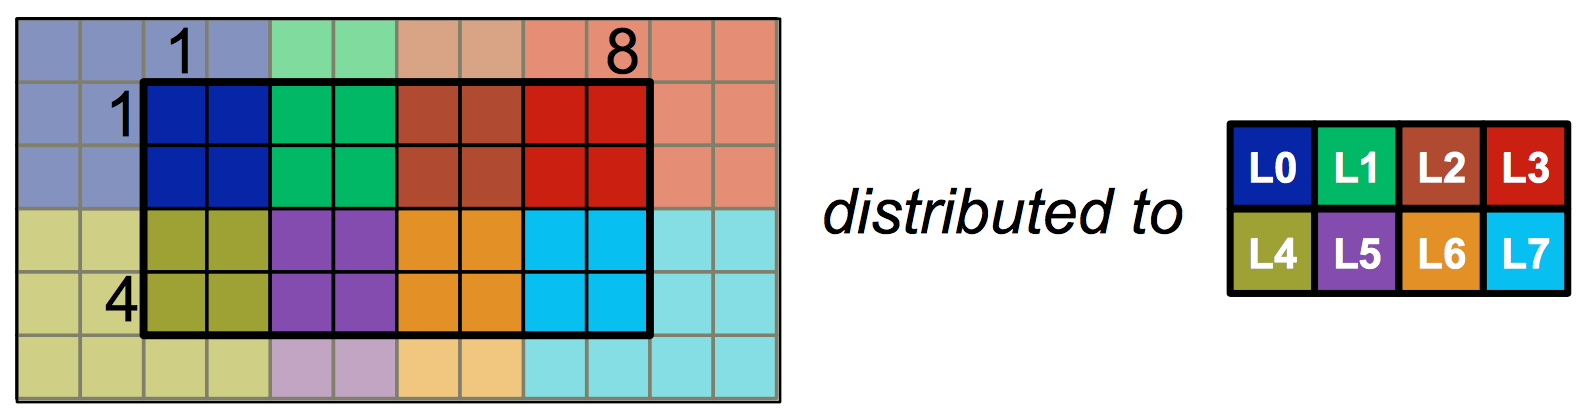
\includegraphics[scale=0.3]{images/blockmap}
			\end{figure}
			\begin{lstlisting}
				var Dom = { 1..4 , 1..8 } dmapped Cyclic( startIdx = ( 1 , 1 ) ) ;
			\end{lstlisting}
			\begin{figure}
				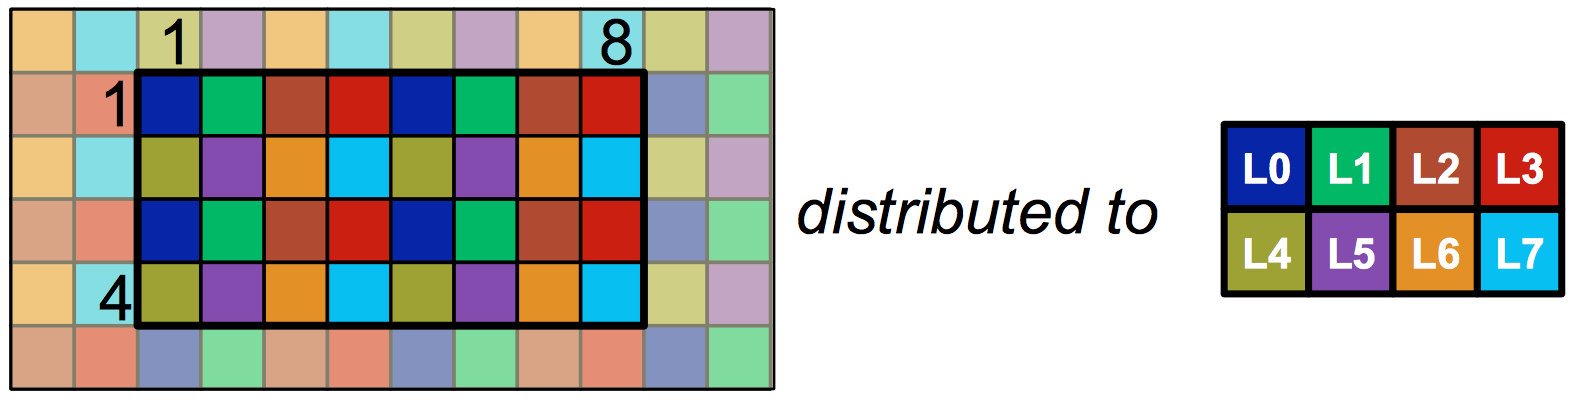
\includegraphics[scale=0.3]{images/cyclicmap}
			\end{figure}
		\end{frame}
		
		% TASK
		\begin{frame}[fragile]{Task Parallelism}
			\begin{block}{Definição}
				\begin{itemize}
					\item Tarefa: Unidade de computação que pode executar em paralelo com outras tarefas
					\item Thread: Recurso do sistema que executa tarefas
				\end{itemize}
				Então, task parallelism é um estilo de programação paralela em que o paralelismo tem tarefas especificadas pelo programador.
			\end{block}
		\end{frame}
		\begin{frame}[fragile]{Task Parallelism}
			\begin{block}{}
				\begin{itemize}
					\item Begin: Executa uma tarefa de forma asíncrona
					\item Cobegin: Executa muitas tarefas em paralelo e espera que todas terminam
					\item Coforall: Cria uma tarefa por cada iteração
				\end{itemize}
			\end{block}
			\begin{lstlisting}
				proc quickSort( arr , low , high ){
				   if( high - low < 4 ){
				      bubbleSort( arr , low , high ) ;
				   }else{
				      const pivot = partition( arr , low , high ) ;
				      cobegin{
				         quicksort( arr , low , p - 1 ) ;
				         quicksort( arr , p + 1 , high ) :
				      }
				   }
				}
			\end{lstlisting}
		\end{frame}
		\begin{frame}[fragile]{Task Parallelism}
			\begin{block}{}
				\begin{itemize}
					\item Sync: Para esperar que a variável tenha um valor quando vai ser usada
					\item Atomic: Cada mudança de valor da variável é atómico
				\end{itemize}
			\end{block}
			\begin{lstlisting}
				var fut : sync real ;
				begin fut = compute() ;
				res = computeSomethingElse() ;
				useComputedResults( fut , res ) ;
			\end{lstlisting}
		\end{frame}
		
		% MULTI-LOCALE
		\begin{frame}[fragile]{Multi-locale Parallelism}
			\begin{block}{Definição}
				Estilo de programação paralela em que o paralelismo é feito em várias máquinas para um mesmo programa
			\end{block}
		\end{frame}
		\begin{frame}{Multi-locale Parallelism}
			Todos os programas em Chapel tem a variável de configuração $numLocales$ e também pode ser modificada ao executar. Além disso, tem a constante $Locales$ que é um array das máquinas configuradas em Chapel.
			Também tem os seguintes métodos para cada locale:
			\begin{itemize}
				\item locale.id: Retorna o índice na constante $Locales$
				\item locale.name: Retorna o nome da máquina
				\item locale.numCores: Retorna o número de cores da máquina
				\item locale.physicalMemory: Retorna a memoria disponível na máquina
			\end{itemize}
		\end{frame}
		\begin{frame}[fragile]{Exemplo}
			A comunicação de dados entre as diferentes máquinas é implícita. Por exemplo, para duas máquinas temos:
			\begin{lstlisting}
				var x , y : real ; // Locale 0
				on Locales( 1 ){ // Send task to Locale 1
				   var z: real ; // Locale 1
				   z = x + y ; // Locale 1 reads from Locale 0
				   
				   On Locales( 0 ) do
				      z = x + y ; // Remote modification of z in Locale 0
				}
			\end{lstlisting}
		\end{frame}